%!TEX root = doe.tex

\section{Using the New Measure}
\label{sec:replications}

No matter how high-tech the tools used to construct a proxy, its value ultimately depends on its usefulness in other applications.
In this section, we demonstrate the DOE score's usefulness in two ways.
First, to show how our better measure of power can generate even more insights than those discussed above, we replicate a well-known test of the bargaining model that treats power as a main variable of interest.
Second, we replicate 18 recent empirical models to show how the DOE score is a better control variable for models that focus on other explanatory factors across an array of dependent variables.
After that, we provide some advice to practitioners on how to decide which measure (or measures) to include.

\subsection{Power, Benefits, and Conflict}

The DOE score's greatest potential lies in its ability to enhance tests of the role of power in international relations.
To that end, we begin our replication analysis by reanalyzing a well-known test of the bargaining model.
Not only does the model fit better when we replace a traditional measure of power with DOE scores, but it also yields substantively different conclusions about the effect of power relations on the likelihood of violent conflict.

\begin{figure}[tp]
  \centering
  \includegraphics{fig-rcnw-expectations}
  \caption{
    \citeapos{reed2008war} graphical summary of their main hypotheses.
  }
  \label{fig:rcnw-expectations}
\end{figure}

\citet{reed2008war} study how the balance of power between two states affects the likelihood of conflict.
They model the chance of interstate conflict as a function of two important parameters: the probability that one state would prevail over the other in a conflict, $p$, and the distribution of benefits between the two states, $q$.
For example, $q$ may capture where a border is drawn between two neighboring states.
Motivated by Powell's \citeyearpar{powell1996stability,powell1999} theoretical model, they hypothesize that the effect of power depends on the status quo distribution of benefits.
If benefits are distributed evenly between two states, conflict is most likely to break out if one state has a preponderance of power.
Conversely, if the status quo disproportionately favors one state, conflict is most likely if there is a balance of power.
Figure~\ref{fig:rcnw-expectations} summarizes these hypotheses.

\citeauthor{reed2008war} test their theory by incorporating proxies of $|q - p|$ and $(q - p)^2$ (both lagged one year) into a model of dispute onset.
Their measure of $q$, the distribution of benefits, is based on United Nations roll call votes.
Like most of the conflict literature---not to mention this article---their measure of $p$, the dyadic balance of power, uses material capabilities.
Specifically, their proxy for $p$ is a normalized cousin of the capability ratio based on differences in CINC scores.\footnote{%
  For details, see footnote 11 of \citet[1211]{reed2008war}.
}
We replicate \citeauthor{reed2008war}'s analysis, replacing the CINC-based measure of $p$ with DOE scores while keeping all other covariates the same.\footnote{%
  We report our replication of their Model 1.
  The results of our replication of their Model 2, which contains additional controls and peace-year splines, are substantively identical.
}
This is an ideal use case for DOE scores, since \citeauthor{reed2008war}, like us, draw from bargaining theory in treating power as the probability of success in an eventual conflict.
The correlation between the original measure of $|q - p|$ and ours is~0.962.
This is higher than the correlation between the capability ratio and DOE scores because we use the same measure of $q$.

\begin{table}[tp]
  \centering
  \input{tab-rcnw}
  \caption{%
    Replication of Table 1, Model 1 of \citet[1213]{reed2008war}.
    The unit of analysis is the dyad-year, and the dependent variable is the onset of a militarized interstate dispute.
    The proportional reduction in loss over the null model comes from 100 repetitions of 10-fold cross-validation.
  }
  \label{tab:rcnw}
\end{table}

Although our measure is similar, we yield substantively different results about the effect of the distribution of power and benefits on the likelihood of conflict.
Table~\ref{tab:rcnw} summarizes the original analysis and our replication.\footnote{%
  We reconstruct \citeauthor{reed2008war}'s measure of $p$ with the latest National Material Capabilities data---the same we use to make DOE scores---so our sample size is slightly larger than in the original paper.
  The substantive and statistical significance of our estimates with the reconstructed measure, reported in the first column of Table~\ref{tab:rcnw}, are the same as originally.
}
As we would expect, given the affinity between the DOE score and the bargaining model's concept of power, the model fit improves significantly when we measure $p$ with DOE scores instead of CINC scores.
Using a \citet{Vuong:1989uf} test, we reject the null hypothesis of equal fit in favor of the DOE-based model fitting better ($Z = 7.80$, $p < 0.001$).
The DOE model is also superior according to the AIC and cross-validation criteria.
Accordingly, we feel comfortable making inferences from the replicated model.

\begin{figure}[tp]
  \centering
  \input{fig-rcnw-gull}
  \caption{
    Replication of Figure 4 of \citet[1213]{reed2008war}, which provides the predicted probability of MID onset as a function of the distribution of power (horizontal axis) and the distribution of benefits (vertical facets), holding democracy and distance at their minimal values.
    Standard errors obtained via a parametric bootstrap.
  }
  \label{fig:rcnw-gull}
\end{figure}

The replicated model not only fits better, but also yields substantively different conclusions about the balance of power and war.
Because of the nonlinear functional form of the model, we follow \citet{reed2008war} in leaning on graphical interpretations.
Figure~\ref{fig:rcnw-gull} plots the predicted probability of a dispute as a function of the balance of power and the distribution of benefits, according to the original model and our replication.
\citet[1212]{reed2008war} cite their results, plotted in the first column, as ``remarkable'' support of the theoretical expectations reproduced here in Figure~\ref{fig:rcnw-expectations}.
They find that neither power parity theory, which predicts conflict between evenly matched states, nor balance of power theory, which predicts conflict when one state holds a preponderance of power, holds unconditionally.\footnote{%
  See \citet[chapter~3]{powell1999} for further discussion of these schools of thought.
}
Instead, \citeauthor{reed2008war} conclude that the power-conflict relationship resembles balance of power theory when benefits are evenly distributed ($q = 0.5$) and power parity theory when benefits are unequal ($q = 0.1$ or $0.9$).

Our replication with DOE scores, plotted in the second column of Figure~\ref{fig:rcnw-gull}, leads us to overlapping but substantively distinct conclusions.
Like the original analysis, we find that the probability of conflict is always minimized when the distribution of benefits matches the distribution of power, or $q = p$.
In addition, our results for the case when benefits are evenly matched are almost identical to \citeauthor{reed2008war}'s.
On the other hand, we never find support, even conditionally, for the power parity theory.
Our model shows that the probability of conflict is always greatest when the difference between $q$ and $p$ is greatest---i.e., when the side with less benefits holds a preponderance of power.
This finding runs contrary to both the theoretical expectations and the empirical findings of \citeauthor{reed2008war}, who claim that $p \approx 0.5$ is the most dangerous distribution of power when benefits are unequally distributed.


\subsection{Capabilities as Control}

In dyadic analyses of conflict, the capability ratio is usually included as a control variable, not one of the independent variables of interest.
Even when power is not a study's main focus, it is important to use the best available proxy for power.
Unless dyadic power relations have no effect on the outcome of interest (in which case proxies for power do not belong in the model), better proxies will capture more residual variation, resulting in greater model fit and more precise inferences.
And if power is a confounding variable---i.e., power relations are correlated with both the key independent variable and the outcome---then the bias of the estimated relationship will be inversely related to the quality of the proxy.
Reducing variance and bias are key concerns for any empirical analyst, so proxy quality matters.

To compare the performance of the DOE score as a control variable to that of the capability ratio, we replicate 18 recent analyses of conflict.
In each replication, we rerun the main model with DOE scores in place of the capability ratio (or other CINC-derived proxy for relative power).
Our main concern is fit: do the models with the DOE score capture more of the variation in the outcome of interest than those with the capability ratio?
In 14 out of 18 cases, the answer is yes, indicating that DOE scores make for a better control variable in typical statistical analyses of conflict.

We constructed the set of replications by looking for empirical analyses of dyad-years (directed or undirected) that included the capability ratio or another function of CINC scores as a covariate.
Each study was published recently in a prominent political science or international relations journal.\footnote{%
  For details, see footnote~\ref{fn:journals}.
}
We examined only studies with publicly available replication data.
If we could not reproduce a study's main result or were unable to merge the DOE scores into the replication data (e.g., because of missing dyad-year identifiers), we excluded it from the analysis.
We also excluded studies that employed duration models or selection models, due to conceptual and technical problems with assessing their out-of-sample performance.
Lastly, we excluded studies in which our measure of expected dispute outcomes would be endogenous, namely those whose dependent variable was MID outcomes---the same data we used to construct the DOE scores---or a closely related quantity.\footnote{%
  The dependent variable of each study is listed in the Appendix.
  In most cases it is the initiation or onset of a dispute.
}
In the end, we were left with the 18 studies listed in Table~\ref{tab:replications}.

For each analysis in our sample, we begin by identifying the main statistical model reported in the paper, or at least a representative one.\footnote{%
  When no main model is apparent, our heuristic is to pick one on the log-likelihood--sample size frontier.
  Details of the model chosen from each paper and the functions of CINC and DOE scores used are in the Appendix.
}
We then estimate two models: the original model, and a replicated model where we replace any functions of CINC scores with their natural equivalents in DOE scores.
For example, if the capability ratio is logged in the original model, we log the DOE scores in the replicated model.
Our main measure of comparative model fit is the \citet{Vuong:1989uf} statistic for the test of the null hypothesis that the original and replicated models fit equally well.\footnote{%
  We employ the standard Bayesian Information Criterion \citep{Schwarz:1978kh} correction to the Vuong test statistic.
  We also measure model fit by the \citet{Akaike:1974ih} Information Criterion and repeated cross-validation; the results, which are reported in the Appendix, are essentially the same.
}

\afterpage{
  \clearpage
  \begin{landscape}
    \begin{table}[h]
      \centering
      \input{tab-replications}
      \caption{
        Summary of results from the replication analysis.
        Positive values of the Vuong test statistic indicate that the model with DOE terms fits better than the model with CINC terms, and vice versa for negative values.
        The next two columns report whether $p < 0.05$ for the main substantive hypothesis test under each model; the final two report whether $p < 0.05$ for a test of the null hypothesis that all power variables have a coefficient of zero.
      }
      \label{tab:replications}
    \end{table}
  \end{landscape}
}

We are also interested in how DOE scores change our inferences about the main substantive variables or about the effect of power itself.
We identify the main substantive hypothesis of each study and perform the corresponding null hypothesis test on both the original model and the DOE score replication.
The hypotheses tested are listed in the Appendix.
To test for an effect of relative power, in the original models we test the null hypothesis that all CINC-derived terms have a coefficient of zero, and in the replication models we do the same with the DOE terms.

Table~\ref{tab:replications} summarizes the results of the replication analysis.
The results further support our contention that DOE scores are superior to the capability ratio as a proxy for relative power.
In a majority of the conflict studies we replicate, we explain more of the variation in the dependent variable when we replace the capability ratio with DOE scores as a control for power.
According to the Vuong statistic, the DOE model fits better in 14 out of 18 cases; in six of these, the difference is statistically significant (the Vuong statistic exceeds 1.96).
These results reinforce our confidence in the DOE score's quality as a proxy for relative power.
They also affirm our conceptualization of relative power as the expected outcome of a dispute: by optimizing for dispute outcome prediction, we end up with a measure that is better for modeling a variety of other outcomes as well.

In most of the replications, the main substantive inference does not depend on the measure of relative power.
That is not surprising, given that power is only a control variable in these studies.
There are two exceptions, both of which are analyses of the international ramifications of domestic politics.
The first is the study by \citet{Arena:2009gk} examining the effects of major powers' government partisanship and economic conditions on their propensity to initiate disputes.
Our replicated model with DOE scores both fits better and leads us not to reject the null hypothesis that government partisanship has zero effect (Wald $\chi^2 = 6.62$, $\text{df} = 8$, $p = 0.58$).\footnote{%
  The null hypothesis is that government partisanship and its three interactions with economic variables have zero coefficient in both the mean and dispersion equations.
  See the Appendix for details.
}
The second is \citeapos{Jung:2014jq} analysis of diversionary conflict.
The original study includes both the capability ratio and a CINC-based measure of rising powers; it interacts the latter with domestic unrest, a key independent variable of interest.
When we replace the capability ratio and the rising power measure with their DOE score equivalents, the resulting model fits better, and domestic unrest and its interaction with rising power are jointly insignificant (Wald $\chi^2 = 3.46$, $\text{df} = 2$, $p = 0.18$).
By using a weak proxy for relative power, both of these analyses fail to pick up its confounding effects on the relationship of interest, leading them to overstate the effects of domestic pressures on international conflict.

The most striking results of the replication analysis come from the tests of the effects of power.
In a third of the original studies, the relative power variables are statistically insignificant.
One might conclude from these results that the importance of material power to international conflict is not robust.
However, the DOE variables are jointly significant in every one of the replicated models.
The insignificance of the capability ratio in many studies is not because power is unimportant, but because the capability ratio is such a poor proxy for power.


\subsection{Advice to Practitioners}

Seeing as neither the capability ratio nor DOE scores are uniformly better in typical applications, how should empirical scholars choose which one to include in their analysis?
Our main recommendation is a theory-driven approach.
When theory provides no guidance, we recommend either a data-driven approach or dropping capability measures altogether.

\begin{figure}[htp]
  \centering
  \input{dag-cap0-doe1}
  \caption{
    Raw capabilities only affect the outcome of interest through the probability of victory.
  }
  \label{fig:dag-cap0-doe1}
\end{figure}

If theory suggests that material capabilities only affect the outcome of interest insofar as they shape the probability of victory, then DOE scores are the best measure to control for.
Figure~\ref{fig:dag-cap0-doe1} contains a causal graph of this situation.
One example of this scenario is the aforementioned test of Powell's~\citeyearpar{powell1996stability,powell1999} theory of by \citet{reed2008war}.

\begin{figure}[htp]
  \centering
  % Main document must include
% \usepackage{tikz}  % for the graphics
% \usepackage{etoolbox}  % for the if-then toggles

\providetoggle{cap-to-dv}
\providetoggle{doe-to-dv}

\toggletrue{cap-to-dv}
\toggletrue{doe-to-dv}

% Main document must include
% \usepackage{tikz}  % for the graphics
% \usepackage{etoolbox}  % for the if-then toggles

\providetoggle{cap-to-dv}
\providetoggle{doe-to-dv}

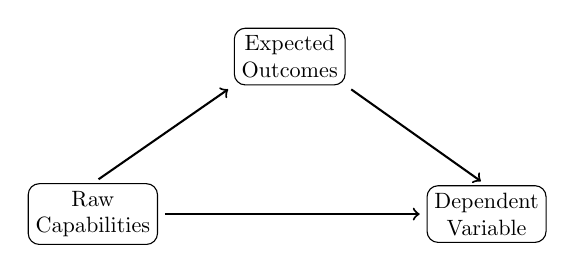
\begin{tikzpicture}[
  var/.style={
    rectangle,
    rounded corners,
    draw=black,
    align=center,
    scale=0.8
    }
  ]
  
  \node[var] (cap) at (0, 0) {Raw\\Capabilities};
  \node[var] (doe) at (2.5, 2) {Expected\\Outcomes};
  \node[var] (dv) at (5, 0) {Dependent\\Variable};

  \path[->, line width=0.75pt] (cap.north) edge[shorten <=0.25em, shorten >=0.25em] (doe.south west);
  \iftoggle{doe-to-dv}{\path[->, line width=0.75pt] (doe.south east) edge[shorten <=0.25em, shorten >=0.25em] (dv.north);}{}
  \iftoggle{cap-to-dv}{\path[->, line width=0.75pt] (cap.east) edge[shorten <=0.25em, shorten >=0.25em] (dv.west);}{}
\end{tikzpicture}

%%% Local Variables:
%%% mode: latex
%%% TeX-master: "doe"
%%% End:


  \caption{
    Raw capabilities affect the outcome of interest both directly and through expectations.
  }
  \label{fig:dag-cap1-doe1}
\end{figure}

If material capabilities affect the outcome both directly and indirectly via victory probabilities, then it would be appropriate to control for both.
Figure~\ref{fig:dag-cap1-doe1} illustrates this scenario.
For example, imagine an empirical study of ``sinking costs'' via military mobilization in international crises \citep{fearon_signaling_1997}.
The initial movement of peaceful relations into a crisis, as well as early behavior at the bargaining table, might be shaped solely by states' expectations about dispute outcomes.
But if states build up their military as a way to signal resolve, independently of the effect on likely outcomes, then raw capabilities matter too.
When empirically modeling a theory like this, scholars should include both DOE scores and raw capability measures.

\begin{figure}[htp]
  \centering
  % Main document must include
% \usepackage{tikz}  % for the graphics
% \usepackage{etoolbox}  % for the if-then toggles

\providetoggle{cap-to-dv}
\providetoggle{doe-to-dv}

\toggletrue{cap-to-dv}
\togglefalse{doe-to-dv}

% Main document must include
% \usepackage{tikz}  % for the graphics
% \usepackage{etoolbox}  % for the if-then toggles

\providetoggle{cap-to-dv}
\providetoggle{doe-to-dv}

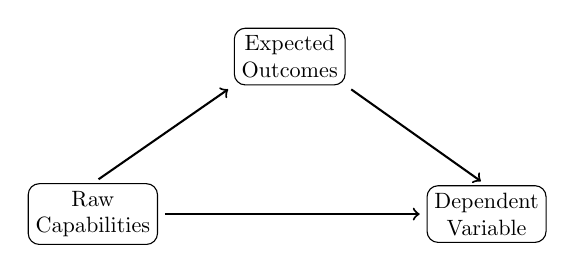
\begin{tikzpicture}[
  var/.style={
    rectangle,
    rounded corners,
    draw=black,
    align=center,
    scale=0.8
    }
  ]
  
  \node[var] (cap) at (0, 0) {Raw\\Capabilities};
  \node[var] (doe) at (2.5, 2) {Expected\\Outcomes};
  \node[var] (dv) at (5, 0) {Dependent\\Variable};

  \path[->, line width=0.75pt] (cap.north) edge[shorten <=0.25em, shorten >=0.25em] (doe.south west);
  \iftoggle{doe-to-dv}{\path[->, line width=0.75pt] (doe.south east) edge[shorten <=0.25em, shorten >=0.25em] (dv.north);}{}
  \iftoggle{cap-to-dv}{\path[->, line width=0.75pt] (cap.east) edge[shorten <=0.25em, shorten >=0.25em] (dv.west);}{}
\end{tikzpicture}

%%% Local Variables:
%%% mode: latex
%%% TeX-master: "doe"
%%% End:


  \caption{
    Raw capabilities directly affect the outcome of interest, but expectations do not.
  }
  \label{fig:dag-cap1-doe0}
\end{figure}

The last possibility to consider is that expectations do not directly affect the outcome of interest.
In this case, empirical models should only include raw capability measures, not DOE scores.
The clearest example is when the dispute outcome itself is the dependent variable.
Because DOE scores are calculated using the dispute outcome data, the DOE scores themselves are endogenous to observed outcomes, and thus should not be included as an independent variable when outcome is the dependent variable.\footnote{%
  In principle, this problem could be solved by only using data for years up to $t-1$ to calculate the DOE score for year~$t$.
  Doing so is not feasible at present given the computational cost.
}

When there is no theory or the theory does not specify how material capabilities affect the outcome of interest, we recommend a data-driven approach.
The steps are the same ones we take in our replication analysis: determine a metric for model fit, run the model separately for each potential measure, and choose the best-fitting model.
Alternatively, if your theory says nothing about the relationship between capabilities and the outcome of interest, it may be best not to include capability measures at all.

%%% Local Variables:
%%% mode: latex
%%% TeX-master: "doe"
%%% End:
